\documentclass[11pt,twoside,a4paper,parskip=full]{scrartcl}
\usepackage{typoday18}

\title{Spiral splines in typeface design}
\subtitle{A case study of Manjari Malayalam typeface}

\author{%
Santhosh Thottingal, Swathanthra Malayalam Computing, santhosh.thottingal@gmail.com\\
Kavya Manohar, Swathanthra Malayalam Computing, sakhi.kavya@gmail.com
}

\begin{document}

\maketitle

\textbf{Abstract}: Manjari typeface was an experiment to use spiral splines to define the curves of Malayalam glyphs. It was a milestone in the progression of script towards maximally rounded glyphs. The script has been evolving from its rectangular characteristics in the early days of metallic types to the circular characteristics of popular digital fonts. The design of curves in Manjari are theoretically based on the PhD thesis by Raph Levien - ``From Spiral to Spline: Optimal Techniques in Interactive Curve Design”. In this paper we present the design principles and aesthetic concepts behind this font. We will also discuss the popularity and adoption of Manjari in the digital as well as print media.

\textbf{Keywords: Malayalam, Script, Spirals, Opentype, Typeface, Digital Typography}

\section{Introduction}

Malayalam script, since its evolution from Brahmi\footnote{\url{https://en.wikipedia.org/wiki/Brahmi_script}} writing style through Vattezhuthu and Grantha\footnote{\url{https://en.wikipedia.org/wiki/Grantha_alphabet}} writing systems to the digital typefaces of modern era, has undergone a lot of changes. The noticeable aesthetic feature of contemporary script is its loops and curly strokes. Horizontal symmetry for many letters like {\manjari{ക, ത, ന}} are a part of script's identity. 

Manjari Malayalam typeface utilises spiral shapes to accentuate these features leading to its aesthetic acceptance. A sample of text rendered in Manjari typeface is shown in Figure \ref{wordcloud}. The use of spiral spline curves resulted in shapes that are extra smooth. The spiral smoothness of curves are complemented by rounded terminals which gives very soft feeling for the eyes. The rigidness of geometric fonts is completely avoided giving a good humanist identity. The curve perfection resulted in negative spaces that acquired beautiful leaf and drop shapes between the bowls and loops of the script. 


\begin{figure}[h!]
	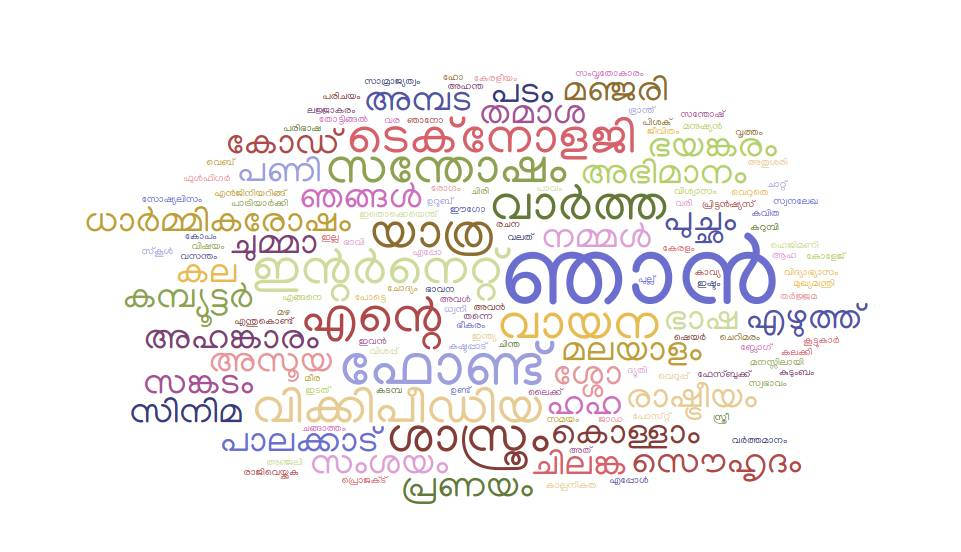
\includegraphics[width=\textwidth]{images/wordcloud.jpg}
	\caption{Text rendered in Manjari typeface}
	\label{wordcloud}
\end{figure} 

\section{Malayalam script}

\subsection{Ancient manuscripts and early printing}

Samples of copper plate inscriptions and palm leaf manuscripts show that the letters were never perfect rounds, but rather rectangular or elongated curves. The sample indicating this is shown in Figure \ref{vattezhuthu} is inscription from Tharisappalli copper plates dating back to 849 AD.


\begin{figure}[h!]
	\includegraphics[width=0.8\textwidth]{images/Tharisappalli_copper_plates.jpg}
	\caption{Copper plate inscription in Vattezhuthu.}
	\label{vattezhuthu}
\end{figure} 

The first ever printed Malayalam book was Samkshepavedartham\cite{samkshepavedartham}, printed in Rome using movable types in 1772. Sample pages of the book is shown in Figure \ref{Samkshepam}. The script was characterized by rectangular features during the early days of printing. 


\begin{figure}[h!]
	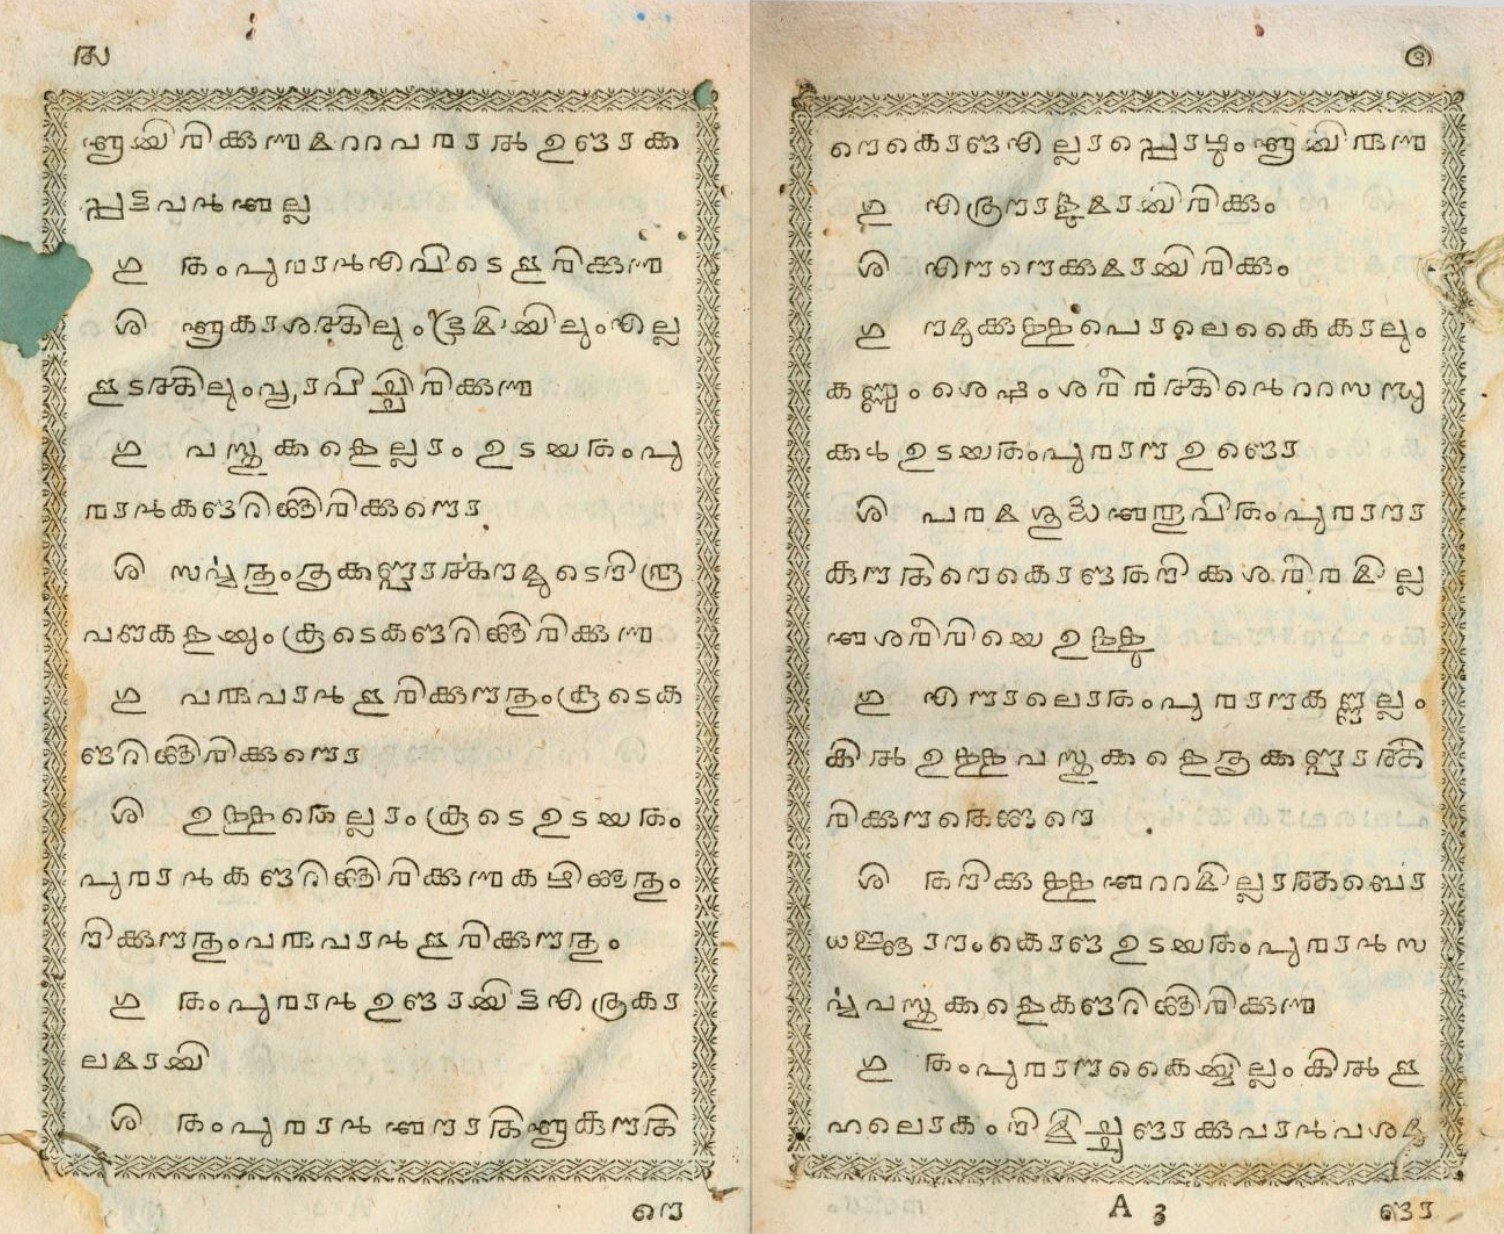
\includegraphics[width=0.8\textwidth]{images/samkshepavedartham1772.png}
	\caption{Samkshepavedartham, 1772. This is the first ever book published Malayalam in movable type. Rectangular nature of glyphs is noticeable}
	\label{Samkshepam}
\end{figure} 

Next remarkable event in history of Malayalam typefaces occurred when movable types were casted natively in Kerala, India during 1829 by an Anglican Missionary Benjamin Bailey\cite{babucherian} for CMS Press, Kottayam, Kerala. These metal types were close to perfect round. The popularity of books from this press started to give uniform height proportions to the script. According to Gupthan Nair, Bailey's contributions as a typographer made the curvy style of the Malayalam script popular\cite{gupthannair}. See the most impactful output from the CMS Press Kottayam in Figure.\ref{newtestament}, a translation of the Bible showing rounded nature of the script.


\begin{figure}[h!]
	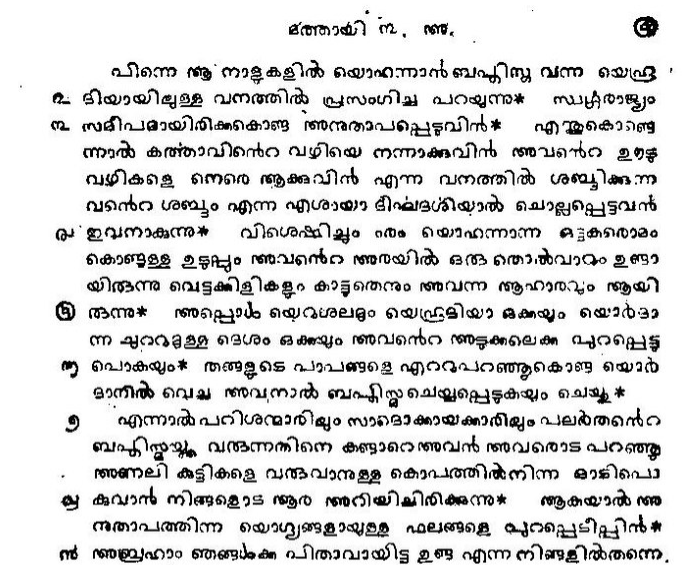
\includegraphics[width=0.8\textwidth]{images/newtestament1829.png}
	\caption{New Testament - 1829}
	\label{newtestament}
\end{figure}

The acceptance of this style of roundness can be easily understood when a fine handwriting is often referred as `{\manjari{അവൾക്കു നല്ല ഉരുണ്ട കയ്യക്ഷരമുണ്ട്} }' (She has a fine round shaped handwriting).

 
\clearpage

\subsection{Digital typefaces}

Digital typefaces of Malayalam script introduced during 1990 that were popular in regular printing were mostly rounded. See Figure.\ref{malsample}. The most popular unicode fonts since their release in the late 2000s, Rachana, Meera and Anjali continued to follow roundness as their glyph characteristic.

\begin{figure}
	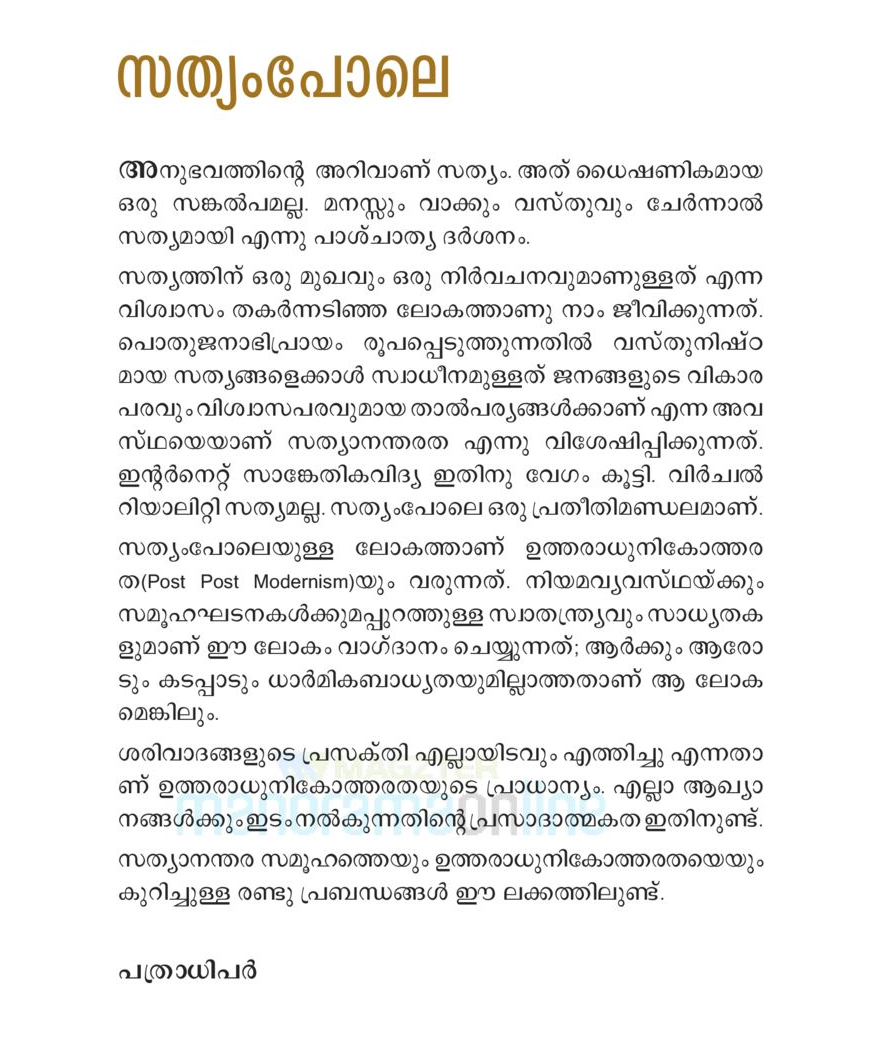
\includegraphics[width=0.6\textwidth]{images/malayalam-sample.png}
	\caption{A sample malayalam rendering to illustrate a common typeface used in printing. Bhashaposhini, February 2018}
	\label{malsample}
\end{figure}

 
Manjari\footnote{Available at \url{https://smc.org.in/fonts/\#manjari}. The source code is published under open font license at \url{https://gitlab.com/smc/manjari}} typeface is designed by Santhosh Thottingal. Opentype engineering was done by Santhosh Thottingal and Kavya Manohar. This font was released in July 2016 and immediately gained wide popularity among Malayalam speakers. The curves in Manjari are designed to follow a spiral shaped path between its control points and the terminals are rounded. %See Figure.\ref{manjari-ka}.

%\begin{figure}
%	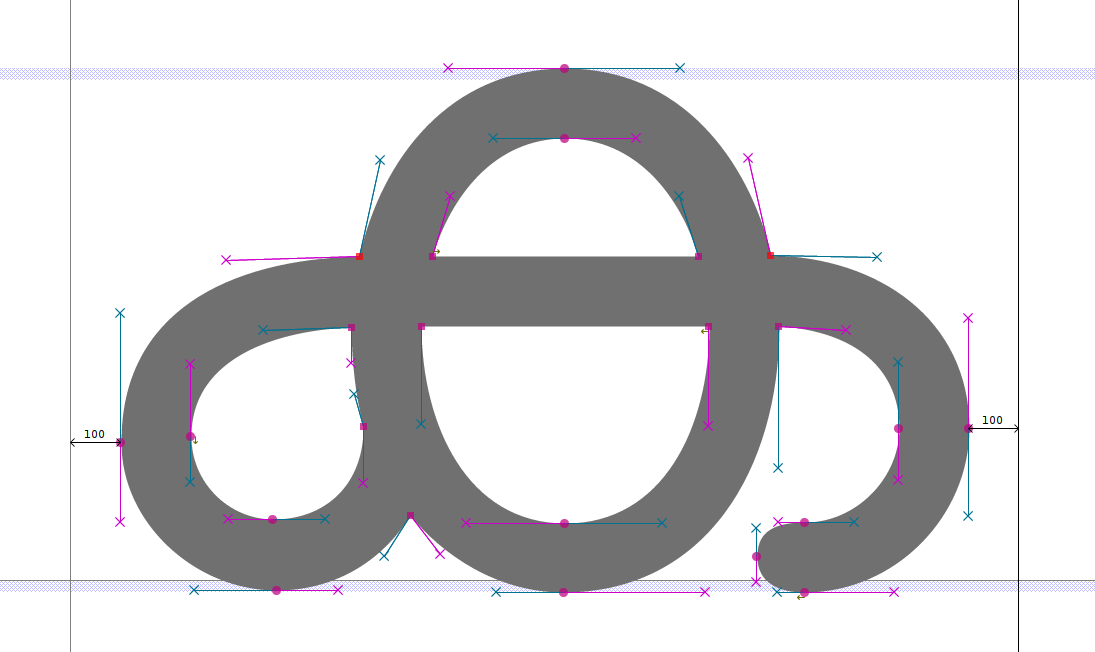
\includegraphics[width=0.8\textwidth]{images/Manjari-Ka.png}
%	\caption{Drawing of letter {\manjari ക} in Manjari font}
%	\label{manjari-ka}
%\end{figure} 
 
\clearpage

\section{Curve Interpolation by Spiral splines}

Curves that passes through control points in a sequence can be termed interpolating splines. A good interpolating spline is a smooth curve that results from sparse control points. There are a huge variety of interpolating curves that include spiral splines, minimum energy curves, log aesthetic curves etc. As mentioned earlier, the nature of smooth interpolating splines have been studied by Ralph levien in his thesis, ``From Spiral to Spline: Optimal Techniques in Interactive Curve Design”\cite{levien}.

According to Levien, spiral spline interpolating curves have certain characteristics which make them particularly suitable for two dimensional curve fitting.
\begin{itemize}
	
	\item \textbf{Roundness Property}: When spiral spline curves are used for interpolation, three data points on a circular path would yield that exact circle after interpolation.
	\item \textbf{Extensionality Property}: When a new control point is introduced on the interpolated spline between two points, the curve shape would be preserved.
\end{itemize}

Geometric continuity is an essential feature indicating the smoothness of interpolating curves between control points. The basic property of connected curves is $G^0$ continuity, ie. curves touch at join points as shown in Figure \ref{g0}. An interpolating curve of better smoothness has $G^1$ continuity, meaning the tangents on either sides of join points are essentially the same as shown in Figure \ref{g1}. 

A still higher order smoothness is offered by $G^2$ continuous curves, having a common center of curvature at the join points as shown in Figure \ref{g2}. Spiral splines can be defined with $G^2$ continuity indicating very smooth variation in curvature. 

\begin{figure}[h!]
	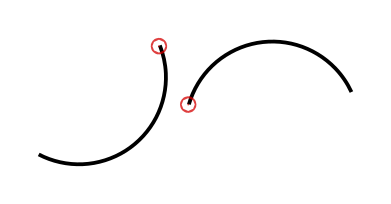
\includegraphics[width=1.0\textwidth]{images/disjoint.png}
	\caption{Disjoint curves. No continuity.}
	\label{disjoint}
\end{figure}

\begin{figure}[h!]
	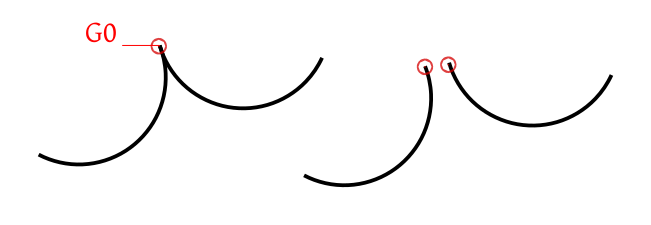
\includegraphics[width=1.0\textwidth]{images/g0.png}
	\caption{$G_0$ continuity. Curves will be continues but there is visible stop point.}
	\label{g0}
\end{figure}

\begin{figure}[h!]
	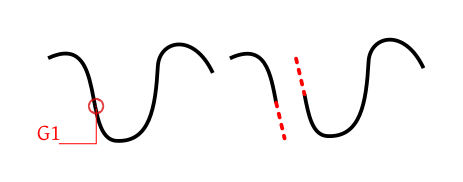
\includegraphics[width=1.0\textwidth]{images/g1.png}
	\caption{$G_1$ continuity. The tangents on either sides of join points are essentially the same. Curves will be appear smooth. But there may be sudden changes in the path.}
	\label{g1}
\end{figure}

\begin{figure}[h!]
	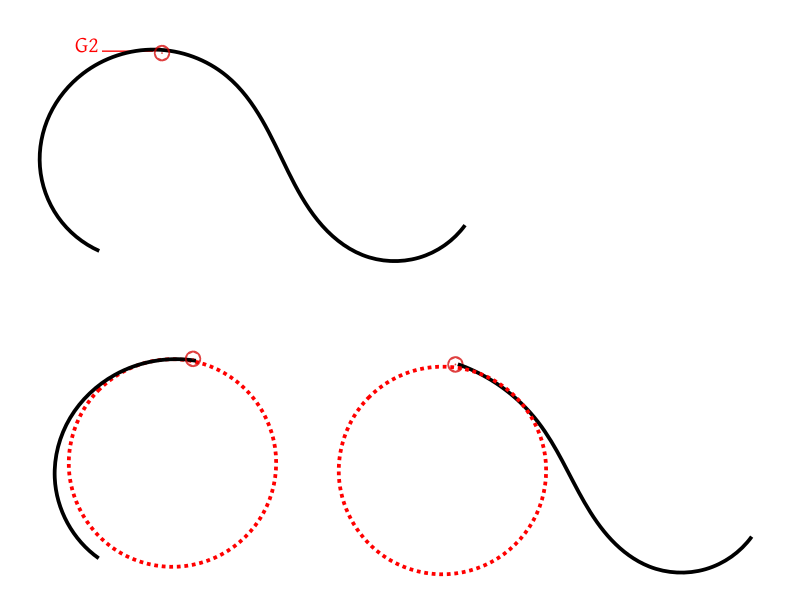
\includegraphics[width=0.8\textwidth]{images/g2.png}
	\caption{$G^2$ continuous curves, having a common center of curvature at the join points. The Spiro library in Inkscape generates $G^2$ curves and same is used for Manjari font.}
	\label{g2}
\end{figure}

Levien proposes that \textit{every curve segment in a two parameter,  $G^2$ continuous interpolating spiral spline between adjacent control points can be cut from an Euler spiral subjecting to rotation, scaling, translation and mirror image transformations}. He calls Euler spiral as the generating curve for spiral splines. Euler spiral has a curvature that changes linearly with its curve length. See Figure \ref{eulerspiral} for a Euler spiral.


\begin{figure}
	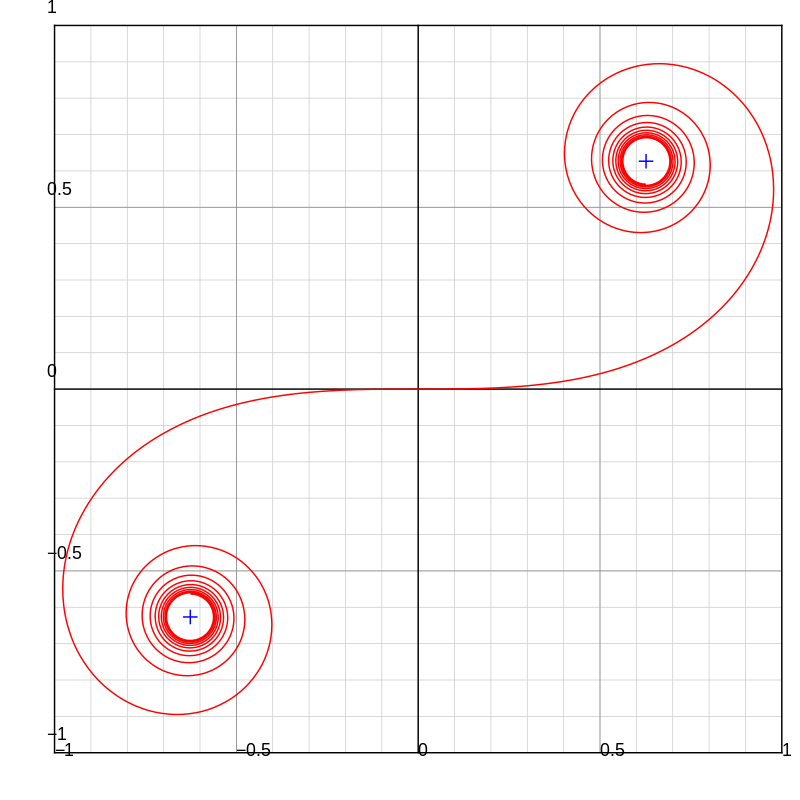
\includegraphics[width=0.8\textwidth]{images/Euler_spiral.png}
	\caption{Euler Spiral, defined by the linear relationship between curvature and arclength, was first proposed as a problem of elasticity by James Bernoulli, then solved accurately by Leonhard Euler}
	\label{eulerspiral}
\end{figure}


The Inconsolata monospace humanist latin font known for its clean lines and elegant design by Levien himself is based on this theory\footnote{\url{http://levien.com/type/myfonts/inconsolata.html}}.

\clearpage

\section{Design process}

The design of Manjari font was done using free software tools in GNU/Linux operating system. The drawing was done in Inkscape using the Spiro tool\footnote{Spiro library. Spiro is a toolkit for curve design, especially font design, created by Raph Levien. It is integrated with Inkscape and Fontforge. \url{http://www.levien.com/spiro/}}, which implements the optimal curve generation technique outlined by Raph Levien. figure \ref{design-1}, \ref{design-2}, \ref{design-3} and \ref{design-4} illustrates the process.

\begin{figure}[h!]
	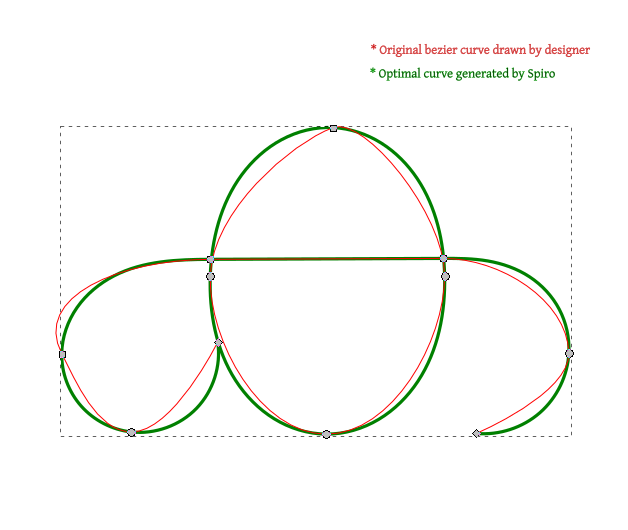
\includegraphics[width=0.8\textwidth]{images/design-1-spiral.png}
	\caption{Designer draws the bezier path. Spiro tool calculates the optimal curve. Designer adjusts the nodes till the glyph shape is achieved.}
	\label{design-1}
\end{figure}

\begin{figure}[h!]
	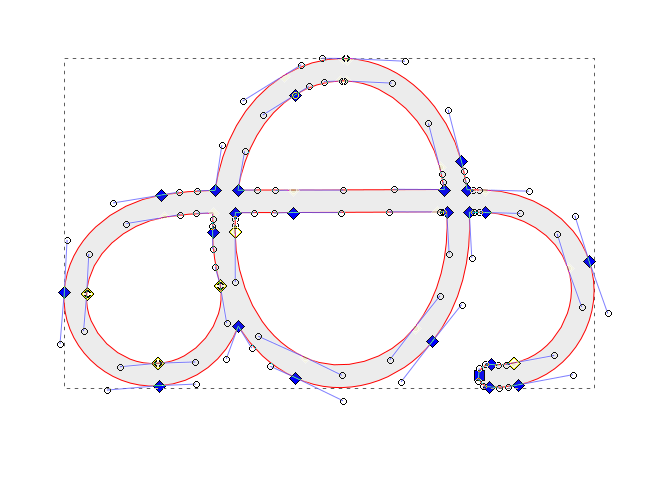
\includegraphics[width=0.8\textwidth]{images/design-2-stroke-to-path.png}
	\caption{The stroke converted to path with desired stroke width. Now this is draft of cubic bezier outline of glyph}
	\label{design-2}
\end{figure}

\begin{figure}[h!]
	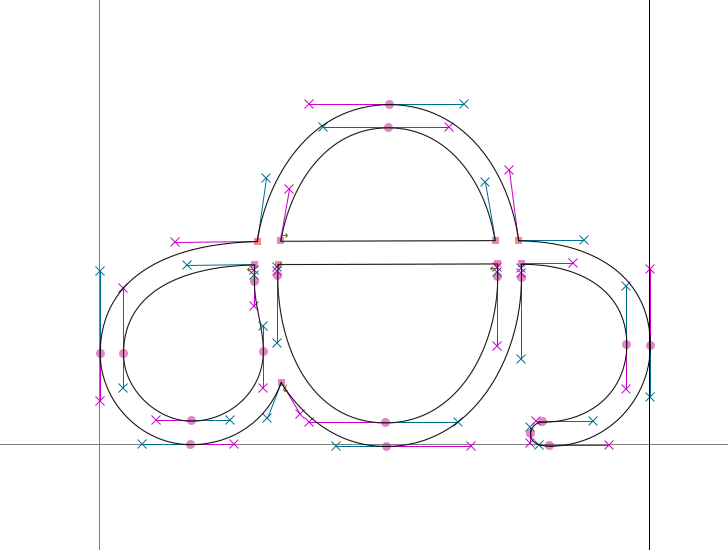
\includegraphics[width=0.8\textwidth]{images/design-3-cubic-bezier-in-font-editor.png}
	\caption{A font editor simplifies and clean up the nodes, defines glyph name, bearings.}
	\label{design-3}
\end{figure}

\begin{figure}[h!]
	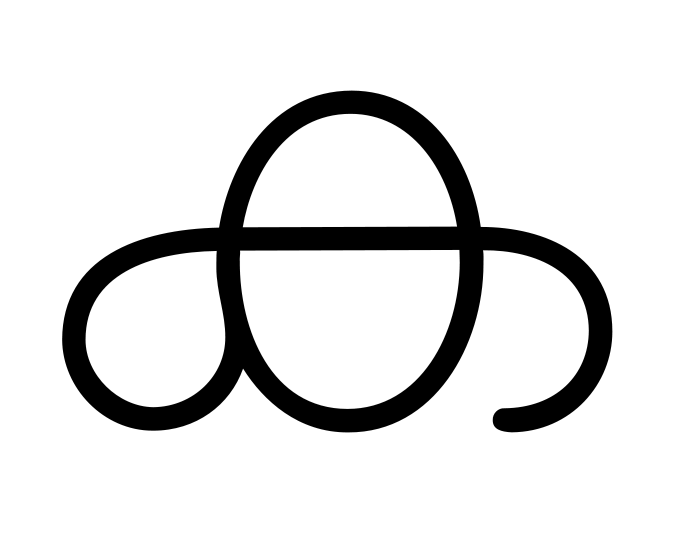
\includegraphics[width=0.8\textwidth]{images/design-4-final.png}
	\caption{Final glyph}
	\label{design-4}
\end{figure}

Manjari is equal thickness typeface. So bold, thin variants prepared by just varying the stroke with in Inkscape, while stroke is controlled by the curves from Spiro. The outline terminals were set to use round shapes, that complements the smoothness in outlines.

The typeface also has a matching Latin character set which follows the same design principles.
\clearpage
\section{Specimen}


\begin{figure}[h!]
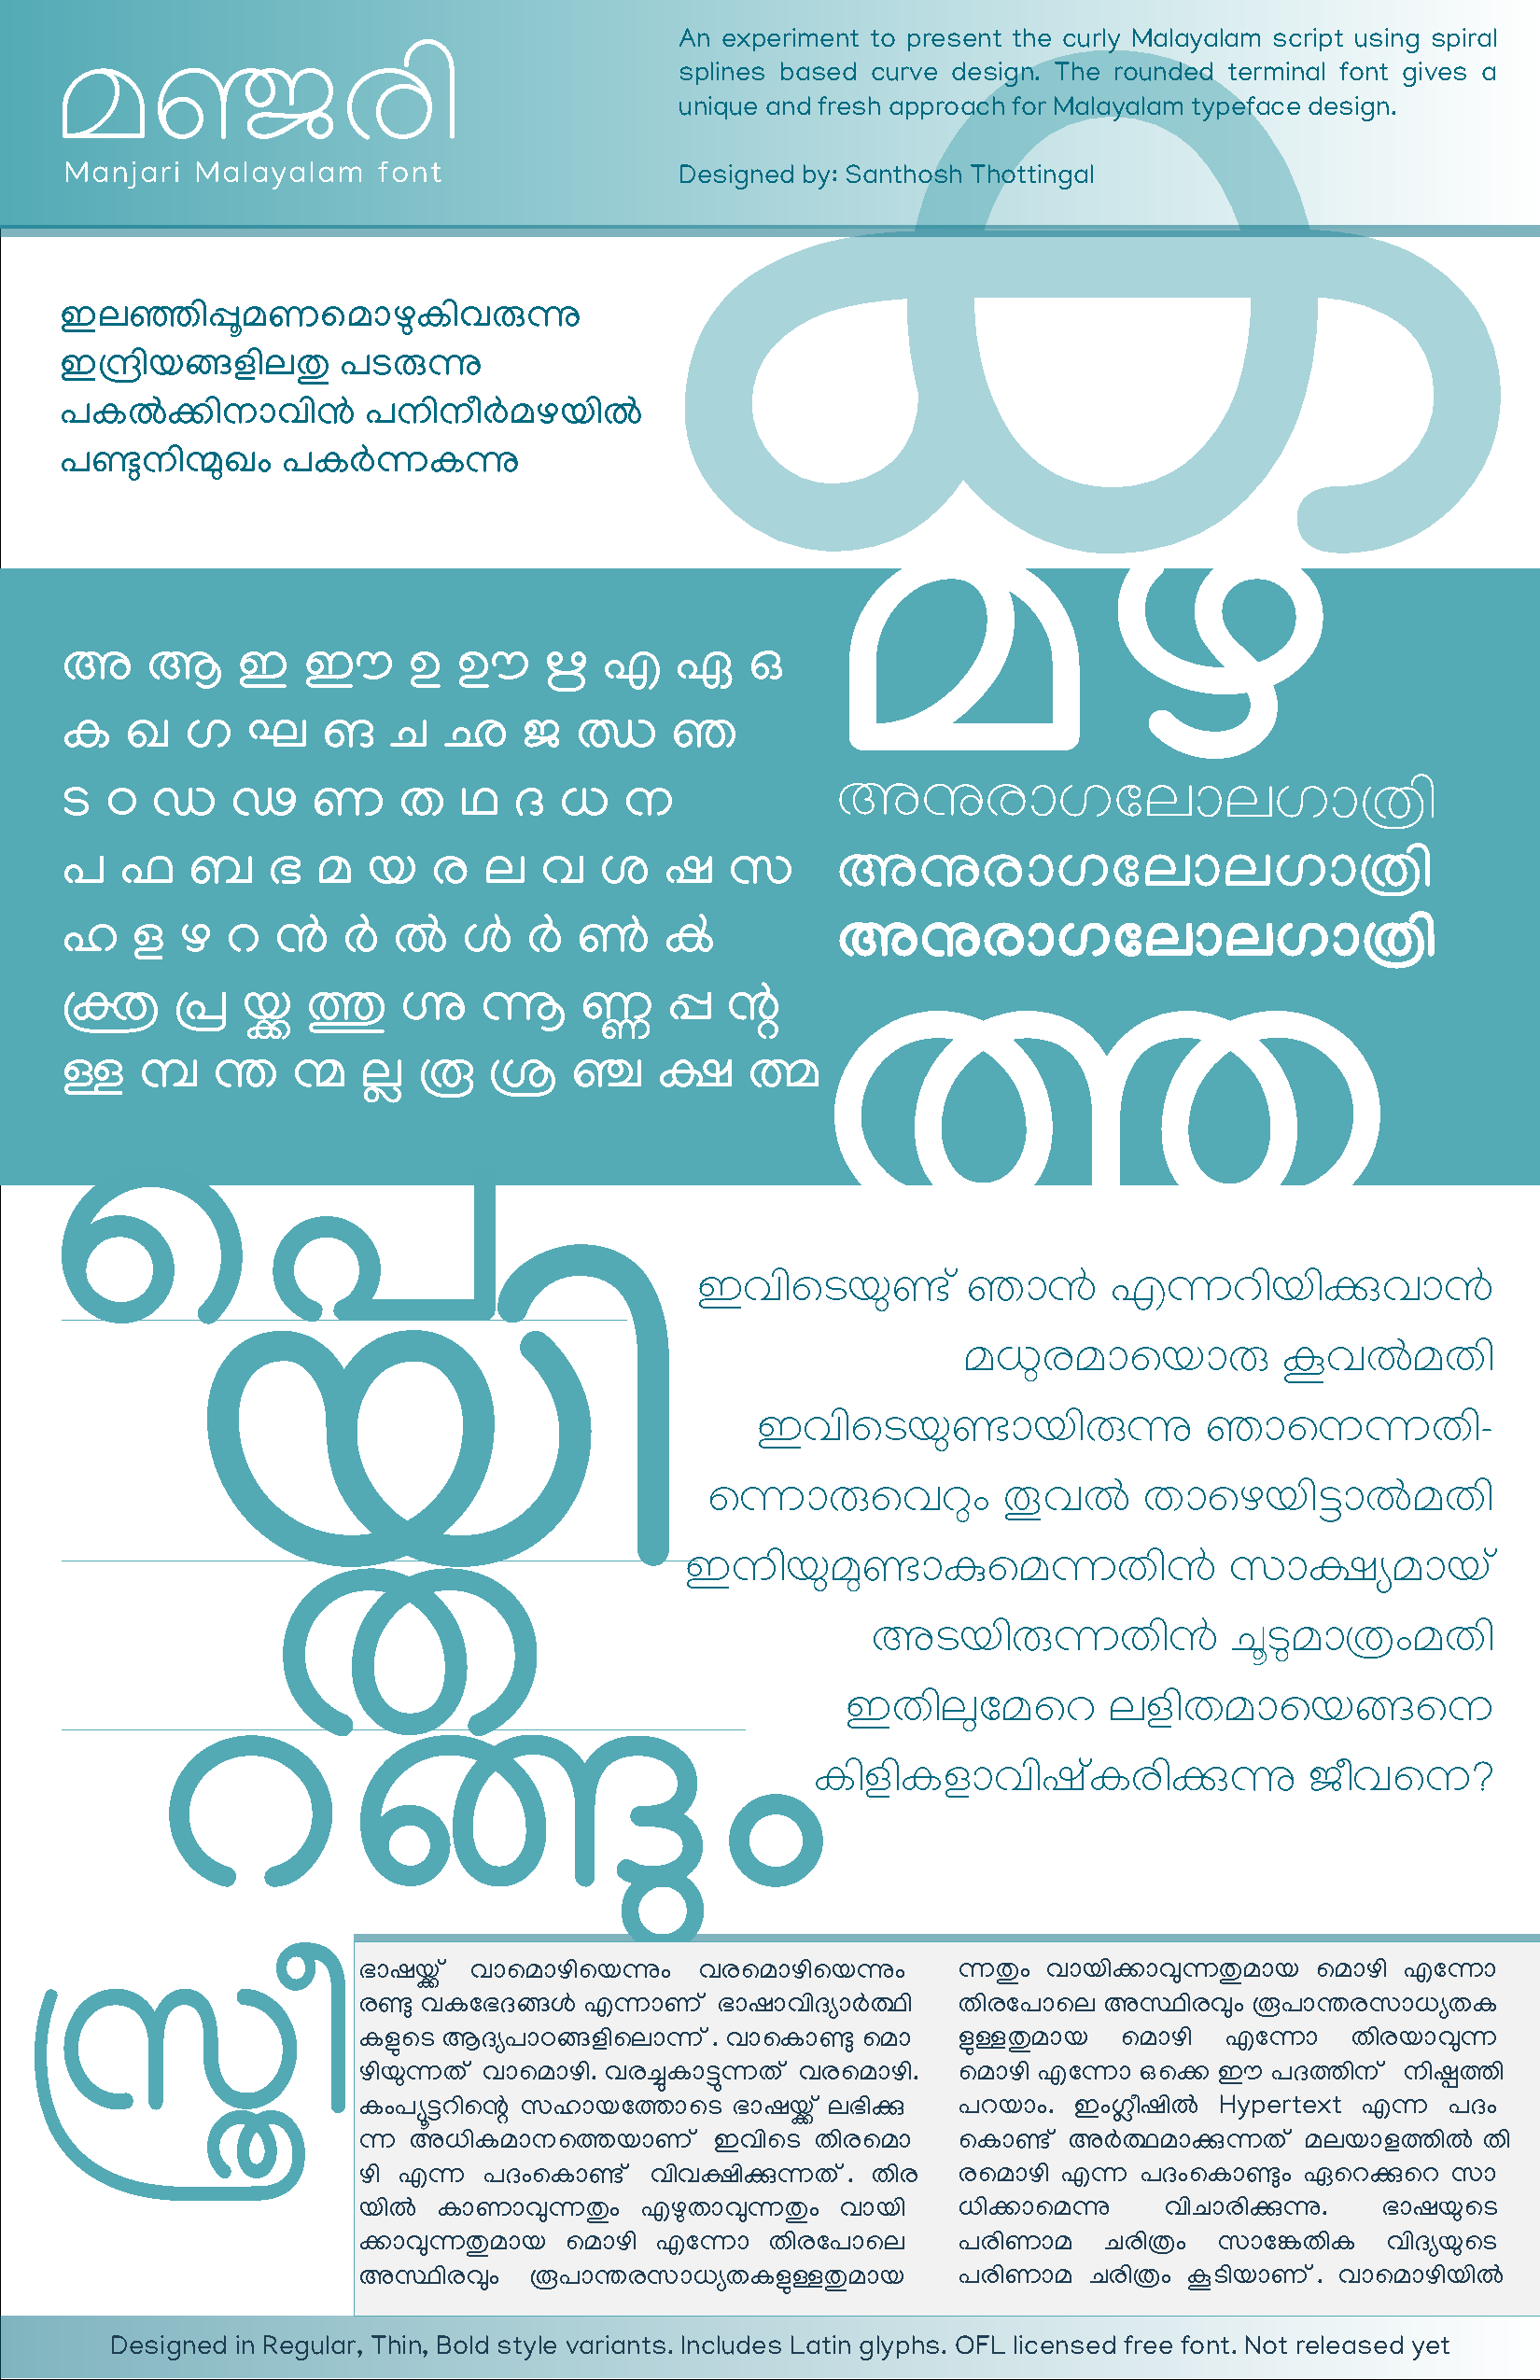
\includegraphics[width=0.9\textwidth]{images/Manjari-Specimen.pdf}
	\caption{A one page specimen of Manjari typeface}
\label{specimen}
\end{figure}
\clearpage

\section{Popularity}

Manjari has gained wide popularity in web as well as print media since in release in July 2016. There are magazines and news portals which use Manjari as a major typeface. Internet memes widely use Manjari. A few samples are shown in Figures \ref{manjari-sample-1}, \ref{manjari-sample-3}, \ref{manjari-sample-4}. 

\begin{figure}[h!]
	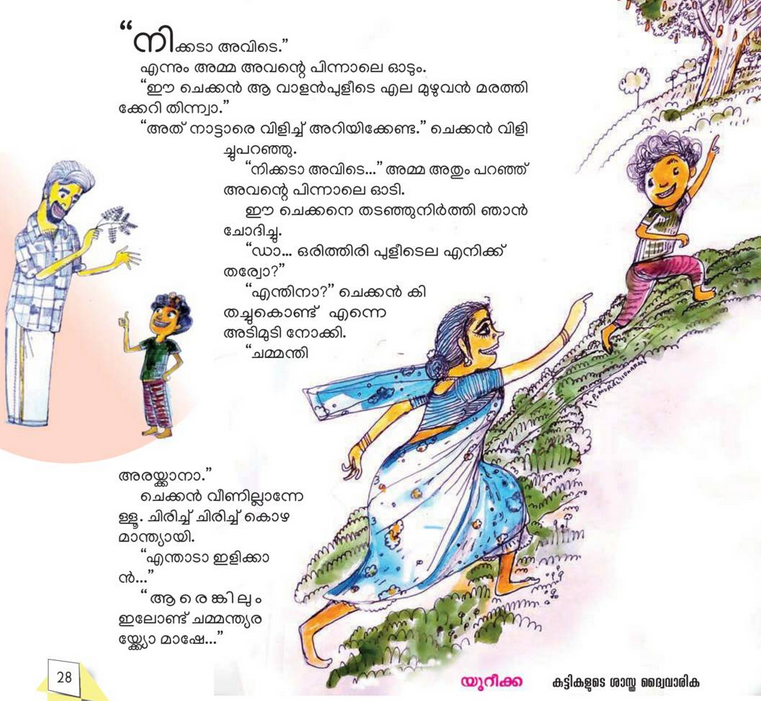
\includegraphics[width=0.8\textwidth]{images/manjari-sample-1.png}
	\caption{A page from `Eureka', Illustrated fortnightly for Children. It uses Manjari for body and titles}
	\label{manjari-sample-1}
\end{figure}




\begin{figure}[h!]
	\begin{subfigure}[b]{.45\textwidth}
		
		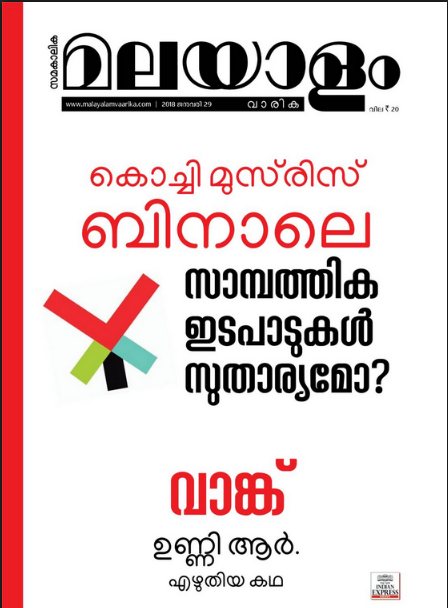
\includegraphics[width=\linewidth]{images/manjari-sample-3.png}
		\end{subfigure}
	\begin{subfigure}[b]{.45\textwidth}
				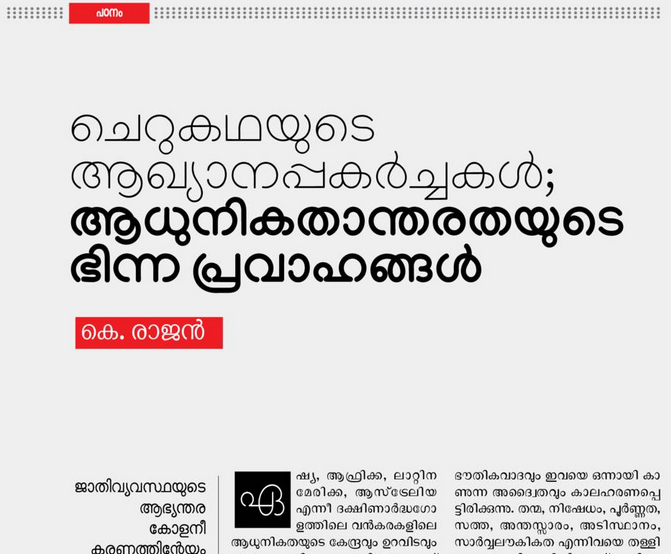
\includegraphics[width=\linewidth]{images/manjari-sample-2.png}
	
	\end{subfigure}

	\caption{'Smakalika Malayalam', Illustrated weekly uses Majari for titles and blurbs}
	\label{manjari-sample-3}
\end{figure}



\begin{figure}[h!]
	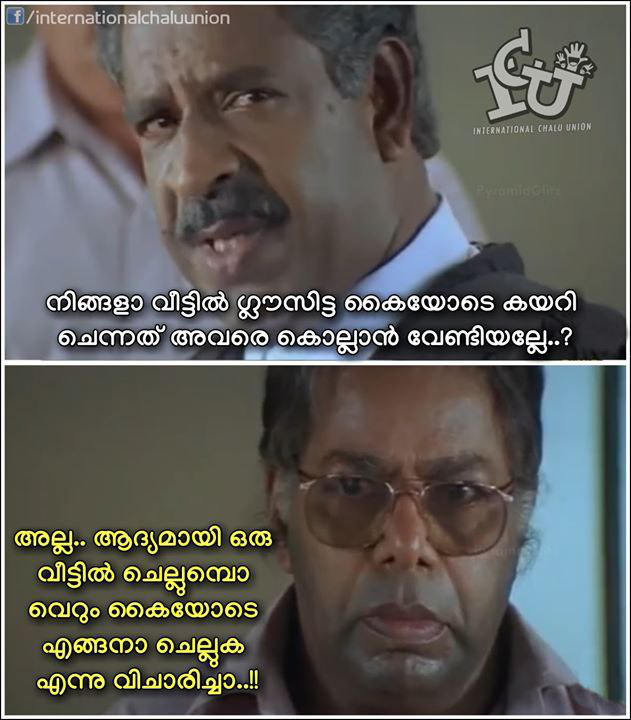
\includegraphics[width=0.8\textwidth]{images/manjari-sample-4.png}
	\caption{An internet meme using Manjari}
	\label{manjari-sample-4}
\end{figure}




\clearpage
\section{Conclusion}

We discussed the design principles and process followed for Manjari typeface. We also discussed how the optimum spiral curve design outlined by Levien is used in the process, which we believe is one of the main factor behind the wide popularity of the typeface is Malayalam.

%\clearpage

\begin{thebibliography}{11}

\bibitem{levien}
  Raphael Linus Levien,
  textit{From Spiral to Spline: Optimal Techniques in Interactive Curve Design},
  EECS Department, University of California, Berkeley,
  2009

\bibitem{samkshepavedartham}
 Clement Pianius,
 \emph{Samkshepa Vedartham},
 \url{https://archive.org/details/SamkshepaVedartham_201311},
 1772

\bibitem{babucherian} Babu Cheriyan, \textit{Benjamin Bailiyum Malayala Sahithyavum} {\manjari{(ബെഞ്ചമിൻ ബെയിലിയും മലയാള സാഹിത്യവും}) }, Mahatma Gandhi University, Kottayam, 2008
	\bibitem{gupthannair} S. Gupthan Nair, \textit{Gadyam Pinnitta Vazhikal}{\manjari{ (ഗദ്യം പിന്നിട്ട വഴികൾ)} }, DC Books, Kottayam 

	
\end{thebibliography}


\end{document}
